\documentclass[10pt, fleqn]{article}

\usepackage{tikz}
\usetikzlibrary{automata, arrows, positioning, fit, petri}

\begin{document}

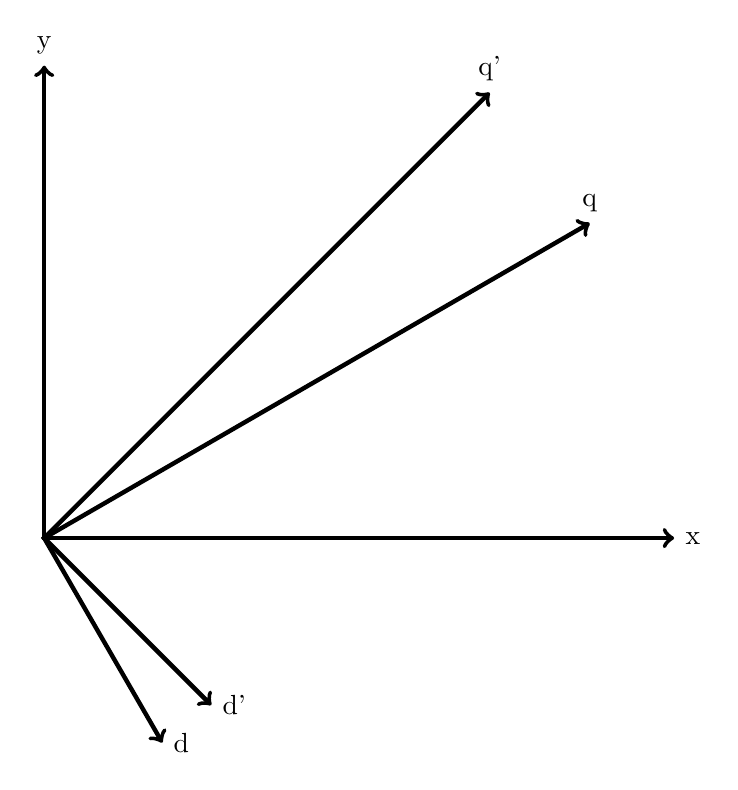
\begin{tikzpicture}[ultra thick, scale = 2]

    \foreach \tilt / \ylength / \xlength / \ylabel / \xlabel in { 0/3/4/{y}/{x}, -45/4/1.5/{q'}/{d'}, -60/4/1.5/{q}/{d} } 
    \draw [<->, rotate=\tilt] (0, \ylength) node (yaxis) [above] {\ylabel} |- (\xlength, 0) node (xaxis) [right] {\xlabel};

\end{tikzpicture}


\end{document}